\documentclass{article}
\usepackage{graphicx}
\usepackage[T1]{fontenc}
% LTeX: language=es
% LTeX: language=en
\usepackage[spanish]{babel}
\graphicspath{ {./resources/} }
\usepackage{float}

\begin{document}

\section{Introducción}

La siguiente guía de instalación busca guiar al usuario en la configuración básica de un laboratorio de Oracle Real Application Clusters, esta guía no busca enseñarle al usuario a utilizar Linux, pero si buscara proporcionar un poco de contexto adicional sobre ciertos comandos de Unix. El laboratorio utiliza 3 máquinas virtuales, las cuales usaran Linux con distribuciones basadas en Ubuntu y RHEL, por otro lado el sistema operativo puede ser cualquiera de preferencia por el usuario, pero en este caso se usará Pop\_Os!, el cual se encuentra basado en Ubuntu.

\section{Configuración de Máquinas Virtuales}

El primer paso consiste en preparar nuestras máquinas virtuales para los nodos de Oracle DB, estos usarán Oracle Linux 7 con Oracle DB 19c, acá cada nodo tiene cuenta con los siguientes requerimientos.

\begin{itemize}
	\item 4 GB de memoria RAM.
	\item 100 GB de almacenamiento físico.
	\item 2 núcleos de procesamiento.
\end{itemize}

Empezando con la creación del primer nodo en este cluster sera llamado ``node1'', aparte de las especificaciones ya mencionadas es necesario crear 3 adaptadores de red:

\begin{itemize}
	\item ``Host-only Adapter'': Usado para conectar à la base de datos hacia otros aplicativos.
	\item ``Internal Network Adapter'': Usado por la red interna del clúster.
	\item ``Bridged Adapter'': Usado para conectarse hacia el internet, usando al sistema operativo huésped.
\end{itemize}

\begin{figure}[H]
	\begin{center}
		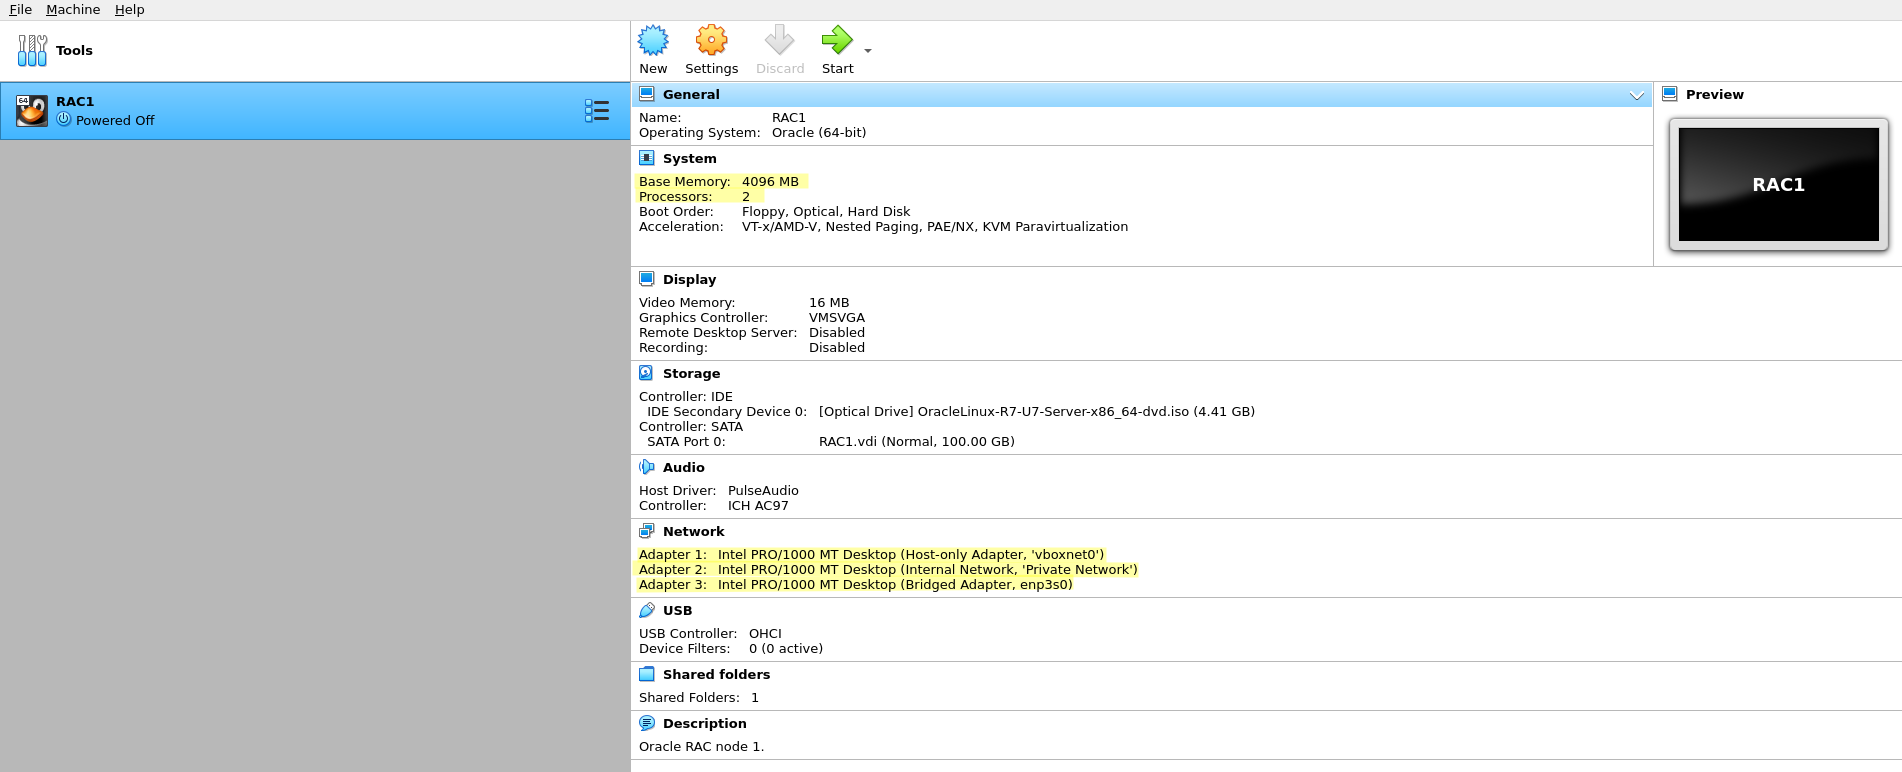
\includegraphics[width=0.95\textwidth]{vm_base.png}
	\end{center}
	\caption{Pantalla de inicio de Configuración de la Máquina Virtual}
\end{figure}

Al momento de iniciar la máquina virtual e insertar el archivo ISO con Oracle Linux 7, podemos empezar a configurar la instalación del sistema operativo. Acá iniciaremos con la configuración de partición del disco desde acá se selecciona ``Installation Destination'', en donde se puede ver el disco creado y las opciones de particiones, acá se seleccionará ``I will configure Partitioning''. Acá crearemos las siguientes particiones.

\begin{center}
	\begin{tabular}{ |c|c|c| }
		\hline
		\multicolumn{2}{|c|}{Lista de Particiones}    \\
		\hline
		Nombre de Partición & Capacidad               \\
		\hline
		/boot               & 2 GB de almacenamiento  \\
		/root               & 5 GB de almacenamiento  \\
		/ o root            & 50 GB de almacenamiento \\
		/swap               & 8 GB de almacenamiento  \\
		\hline
	\end{tabular}
\end{center}

Al volver al menú de inicio de nuestro instalador, se selecciona el software por instalar en nuestra nueva instalación, acá se selecciona la opción ``Software Selection'', acá se puede escoger entre varios ambientes, pero se seleccionará ``Server with GUI'' con los siguientes paquetes de software.

\begin{itemize}
	\item ``Hardware Monitoring Utilities''
	\item ``Large Systems Performance''
	\item ``Network file system client''
	\item ``Performance Tools''
	\item ``Compatibility Libraries''
	\item ``Development Tools''
\end{itemize}

Al volver al inicio del instalador se puede configurar las opciones de red en ``Network and Hostname'' para configurar los adaptadores de red instalados en las máquinas virtuales. 

Después de habilitar el primer adaptador de red, seleccione ``Configure'' y en la pestaña de ``ipv4'' se usara la dirección IP ``192.168.24.1/24'' con una salida de ``0.0.0.0''  manualmente.

\begin{figure}[H]
	\begin{center}
		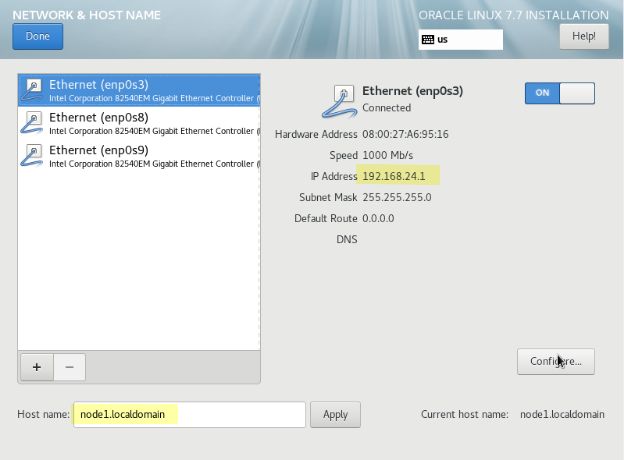
\includegraphics[width=0.95\textwidth]{vm_networking.png}
	\end{center}
	\caption{Configuración de Red de la Instalación de Oracle Linux}
\end{figure}

Se aplicará esta misma configuración manual en el siguiente adaptador disponible, pero esta vez con una dirección IP de ``192.168.10.1/24'' con una salida de ``0.0.0.0'', finalmente para el último adaptador habilitaremos direccionamiento automático con DHCP. Se puede continuar con la instalación del sistema operativo, en la siguiente pantalla podemos seleccionar una contraseña para el usuario ``sudo'', para este ejercicio se usará ``root'' como contraseña.

\end{document}
